\section{Setup and conventions}

\begin{itemize}
\item \textbf{Layout} (since 5 Nov 2026): FairShip \texttt{geometry\_config.py} 2026-0.1 in the target-aligned frame
$z_\text{veto}=z_\text{FS}-2.14$\,m: shield end 29.89\,m, vessel 31.13--81.13\,m (UBT on the entrance window),
straw stations 82.08 / 84.08 / 91.08 / 93.08\,m, timing detector 94.01\,m ($5.5\times6.5$\,m), spectrometer magnet
84.36--89.56\,m. Stored muon states stay at 30.6 / 82.0\,m; every crossing is computed from them. Results older than
5 Nov use the old layout. \src{ISSUES.txt GEOMETRY}
\item \textbf{Normalisation}: $4\times10^{13}$\,\pot{} per spill everywhere (D13, legacy inputs rescaled when read),
15\,y = $1.5\times10^7$ spills. Flat 1\,s spill (A5).
\item \textbf{Muon source}: \texttt{target-production-complete-november-4-2026} (FairShip target, Pythia 8.223,
Geant4 11.2 FTFP\_BERT, every muon source forced and weighted, 10\,GeV threshold), validated against unforced
production (27 species within $2\sigma$, full events $1.003\pm0.005$) and reproducing the 2018 FairShip files to
1--3\,\% once FairShip's 2018 weighting is applied (Fig.~\ref{fig:source}). The 2018 files lack $\sim22$--24\,\% of the
physical flux ($\eta\to\mu\mu\gamma$, $\omega\to\pi^0\mu\mu$). \src{docs/STATUS.md (1 Nov, 4 Nov)}
\item \textbf{Muon flow per spill}: $4.69\times10^{10}$ from the target, $4.38\times10^{10}$ stop in the shield,
$3.11\times10^{9}$ reach 30.6\,m ($1.46\times10^9$ into the $-x$ wall, $9.1\times10^7$ into the floor),
$\sim3\times10^{4}$ reach SST1. \src{docs/STATUS.md (2026-11-08)}
\item \textbf{Transport}: cuda-muons (TRY6 shield, field, rock), shell storage around the vessel (3\,780 seeds).
\item \textbf{MS7 chain default}: Geant4 11.2 muonNuclear (D3 decision of 9 Nov); Pythia 6 / Pythia 8 as the generator
systematic.
\item \textbf{Selection}: $\ge2$ good tracks at SST1, fiducial, measured IP $<10$\,cm (fully reconstructed) or
$<2.5$\,m (partially reconstructed); veto levels b (reconstructed hits) and c (truth).
\end{itemize}

\begin{figure}[h]
\centering
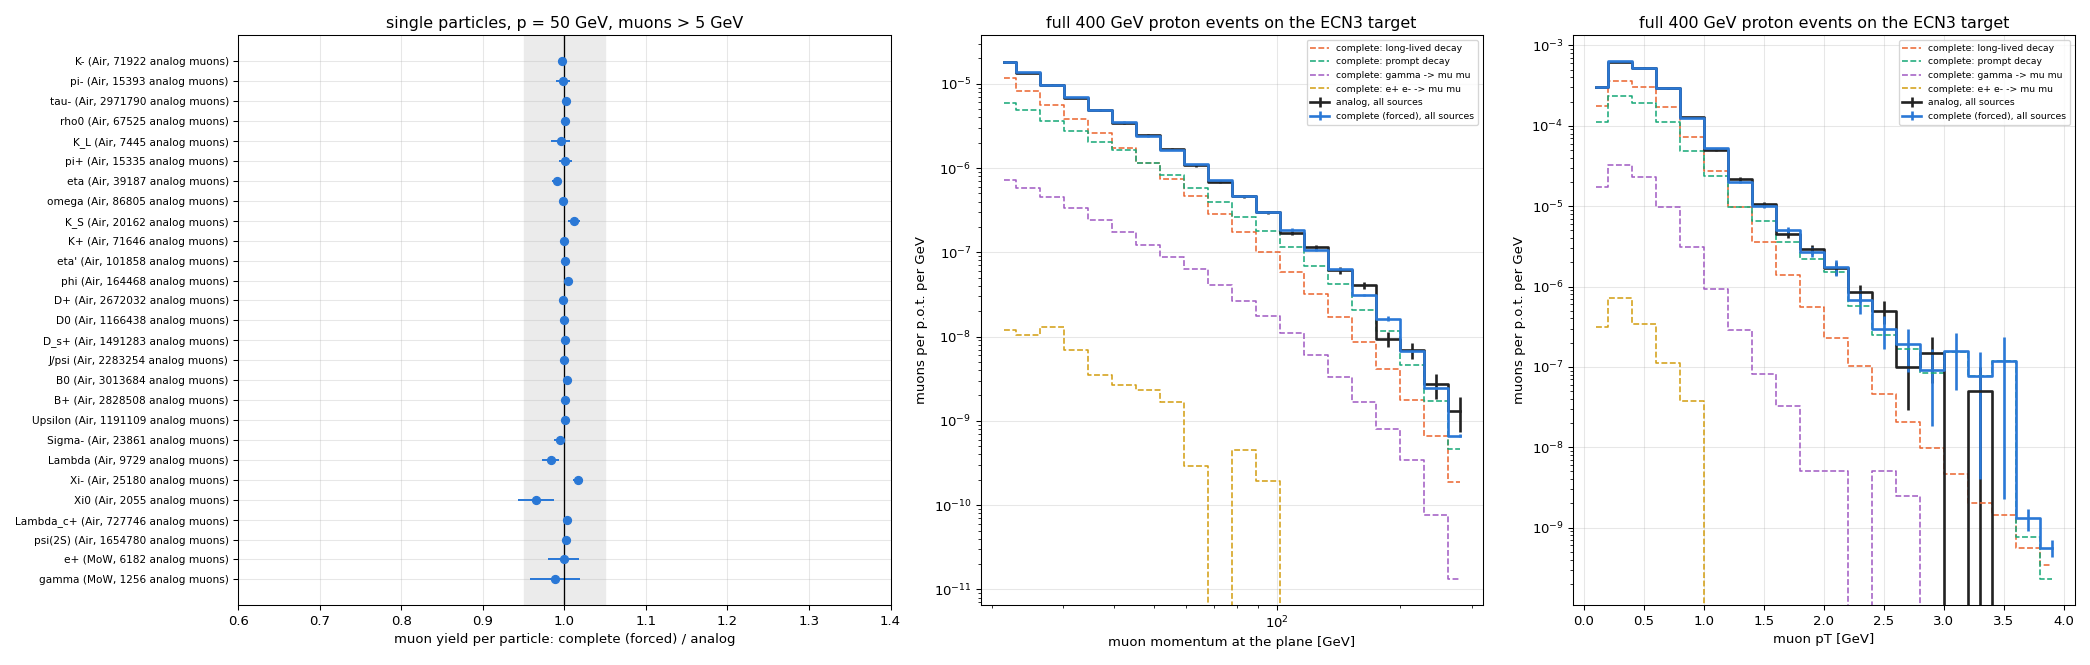
\includegraphics[width=\linewidth]{complete_validation.png}
\caption{Validation of the complete target production (forced vs analog, per species and full events).
\src{lhcb_data .../results/complete_validation/complete_validation.png}}
\label{fig:source}
\end{figure}
